% !TeX root = ../../Thesis.tex
\chapter{Effects of an External Magnetic Field on Stimulated Raman Scattering}
\label{chp:magSRS}

In this chapter, we present work performed while employed as a Junior Specialist at the University of California, San Diego between January and April 2020. The project was supervised by Professor Farhat Beg, and lead by Dr Adam Higginson (now at University of Boulder). The work presented (including data generated and data analysis) was carried out by the author, except in the cases outline below:
\begin{itemize}
\item Figure \ref{fig:SRS_LULI} SRS reflectivity from LULI, made by Matthieu
\end{itemize}

The chapter begins with a review of the literature which discusses the effect of an externally-applied magnetic field on stimulated Raman scattering. We then present modelling, performed by the author, of an experiment performed on the LULI laser system in France by: J. R. Marqu\`es, P. Loiseau, J. B\'eard, A. Castan, B. Coleman, T. Gangolf, L. Lancia, A. Soloviev, O. Portugall, and J. Fuchs. Analysis of the SRS diagnostics was performed by J. R. Marq\`es, and (revisited) by M. Bailly-Grandvaux.  The experiment showed a small increase in SRS with an applied magnetic field, and this is recreated in our simulations. We then go on to investigate how the effect of the magnetic field depends on $\kld$ of the SRS electron plasma wave.

N.B. In this section, all simulations are driven by a $1\omega$ Nd:glass laser with $\lambda_0$. This is different to Chapter \ref{chp:iSRS}, which used the third harmonic of Nd:glass ($\lambda_0=351\si{\nano\metre}$) and Chapter \ref{chp:broadbandSRS} which 

\section{Motivation and literature review}

Once again, wjhy is this a problem? why can we model in 1D? 

How can we continue to only consider modes without B field? Why no X or O modes?

\subsection{Magnetic field suppresses kinetic SRS}

here's a recent paper about 90T fields effect on SRS in inhomogeneous plasmas \citep{Zhou2021}. 

Start by replicating results from \cite{Winjum2018}



Suppress SRS to reduce harmful electrons and reflectivity, or enhance if it actually makes good electrons (in the case of shock-ignition)

\subsection{Magnetic field could enhance kinetic SRS}

\subsection{What about fluid SRS?}

\section{Modelling SRS on LULI}
\subsection{Experimental results}
\begin{figure}[ht]
   \centering
    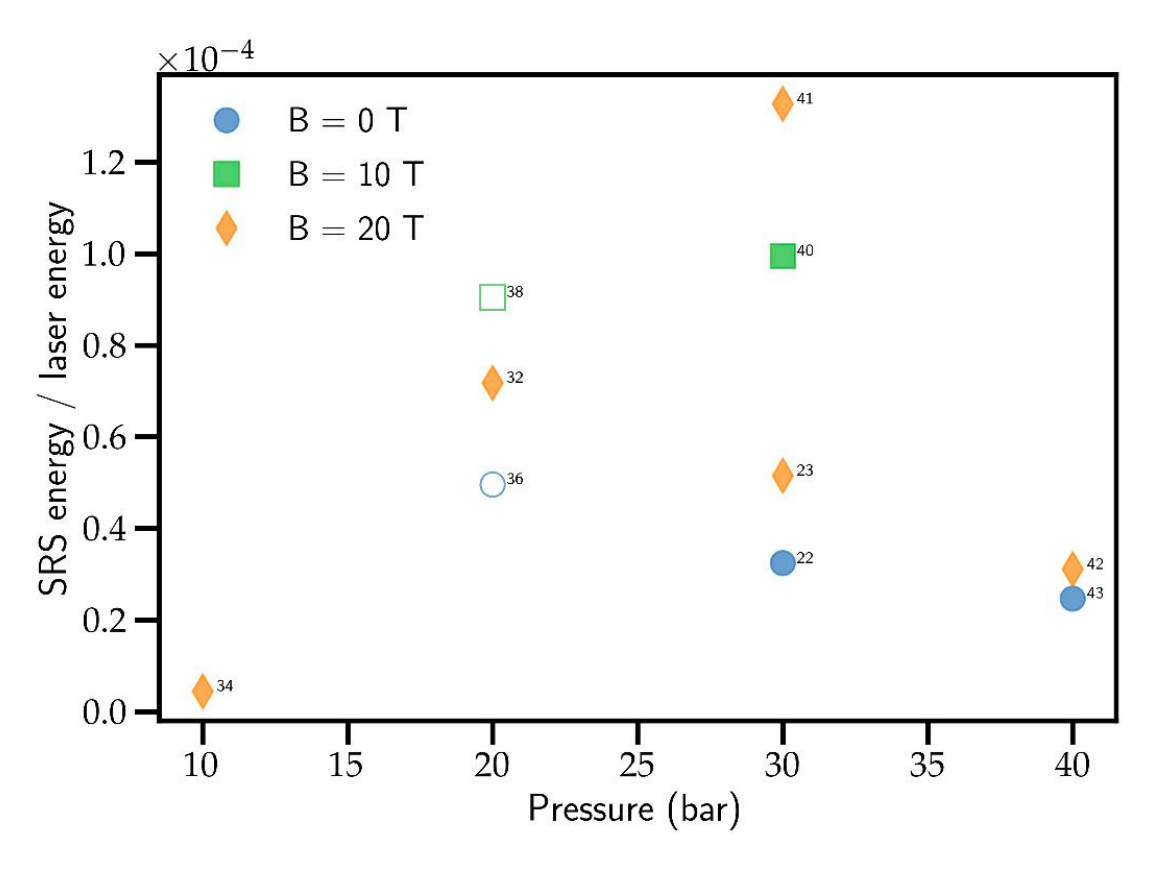
\includegraphics[width=0.8\columnwidth]{Chapters/C6_magSRS/SRS_LULI.png}
    \caption{Experimentally-measured SRS energy at different gas jet pressures, with and without magnetic fields. The solid-coloured markers represent shots with the laser  horizontally polarised with respect to the applied magnetic field, so that the laser magnetic field and applied magnetic field are parallel. The un-filled markers represent vertical polarisation of the laser.}
    \label{fig:SRS_LULI}
\end{figure}{}


\subsection{Simulation results}

Plasma density and temperature profiles at the centre of the gas jet were simulated using the FLASH code by Adam Higginson. 

\begin{table}[h]
\begin{center}

\begin{tabular}{|l|l|l|l|}
\hline
$n_e$ / $n_{\mathrm{cr}}$ & $T_e$ / eV & bSRS $\kld$ & fSRS $\kld$\\ \hline \hline
0.01 & 180 & 0.36 & 0.02 \\ \hline
0.025& 450 & 0.34 & 0.03 \\ \hline
0.05 & 600 & 0.27 & 0.04 \\ \hline
0.10 & 900 & 0.21 &  0.05\\ \hline
0.15 & 1100 & 0.18 & 0.06 \\ \hline

\end{tabular}

\end{center}
\caption{$T_i$ is $T_e/3$ in all cases}
\label{tab:LULI_setup}
\end{table}


\begin{figure}[ht]
   \centering
    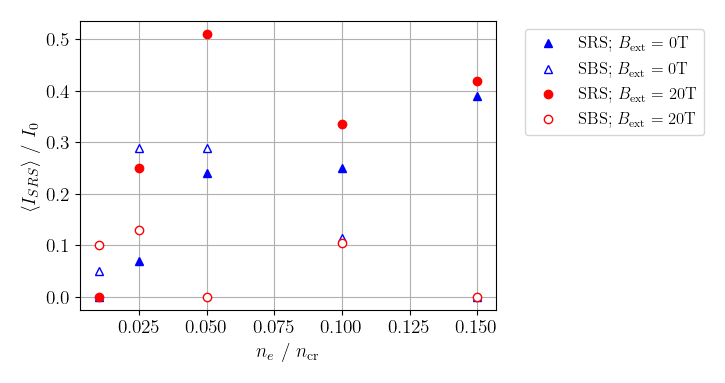
\includegraphics[width=\columnwidth]{Chapters/C6_magSRS/LULI_sims_v3.png}
    \caption{MAthieu made this}
    \label{fig:LULI_sims_v3}
\end{figure}{}



\section{Magnetic field effect varies with plasma debye length}

\citep{Feng2018} REALLY good reference about SRS and LDI and anti-LDI

also don't forget this great paper about kld scling of iSRS autoresonance \citep{Chapman2013}

\subsection{Fixed ions: vary $\kld$}

Plasma parameters chosen to be relevant to LULI experiment (ish). $\lambda_0 = 1053 \si{\nano\metre}$; $L_x = 1000 \si{\micro\metre}$; $T_e = 1 \si{\kilo\electronvolt}$; $I_0 = 1\times 10^{15}\si{W/\cm^2}$; $T_{\mathrm{end}}=10 \si{ps}$; 1000 PPC (from convergence testing on $\left< I_{\mathrm{SRS}} \right>_{t>0}$).

\begin{table}[h]
\begin{center}

\begin{tabular}{|l|l|l|l|}
\hline
$n_e$ / $n_{\mathrm{cr}}$ & $\kld$ & regime & predicted behaviour\\ \hline \hline
0.02 & 0.55 & beyond ``loss of resonance" & no SRS, no dependence on $B_{\mathrm{ext}}$  \\ \hline
0.05 & 0.33 & strongly kinetic &  \\ \hline
0.08 & 0.25 & kinetic &  \\ \hline
0.11 & 0.20 & weakly kinetic & \\ \hline
0.20 & 0.12 & fluid & no dependence on $B_{\mathrm{ext}}$\\ \hline

\end{tabular}

\end{center}
\caption{Plasma density, $\kld$, regime, predicted behaviour}
\label{tab:predictions}
\end{table}

\begin{figure}[ht]
   \centering
    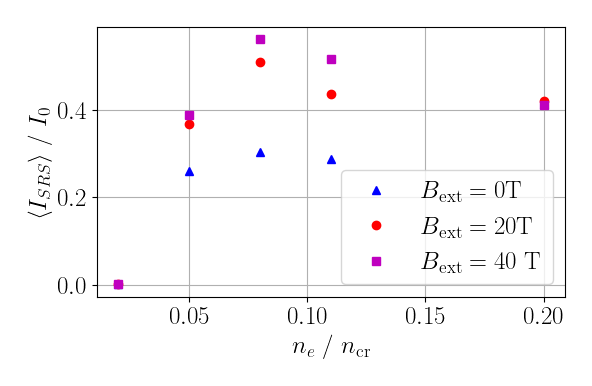
\includegraphics[width=0.9\columnwidth]{Chapters/C6_magSRS/kld_scan_SRS_scaling.png}
    \caption{I made this. Parameters constant to all sims: 
 $\lambda_0 = 1056 \si{\nano\metre}$; $L_x = 1000 \si{\micro\metre}$; $T_e = 1 \si{\kilo\electronvolt}$; $I_0 = 1\times 10^{15}\si{W/\cm^2}$; $T_{\mathrm{end}}=10 \si{ps}$; 1000 PPC.}
    \label{fig:SRS_EPOCH}
\end{figure}{}


\section{Magnetic field effect changes with polarisation}




